\documentclass[]{article}
\usepackage{graphicx}
\usepackage[margin=1cm]{geometry}
\usepackage{csvsimple}
\usepackage{hyperref}

\begin{document}
\listoffigures
\listoftables

\newpage
\section*{\centering $ 0.3 < p_T < 1.5$ and $ |\eta|<1$}
\subsubsection*{\centering All NPOMS and NPOMH=0}

\begin{figure}[h!]
    \centering
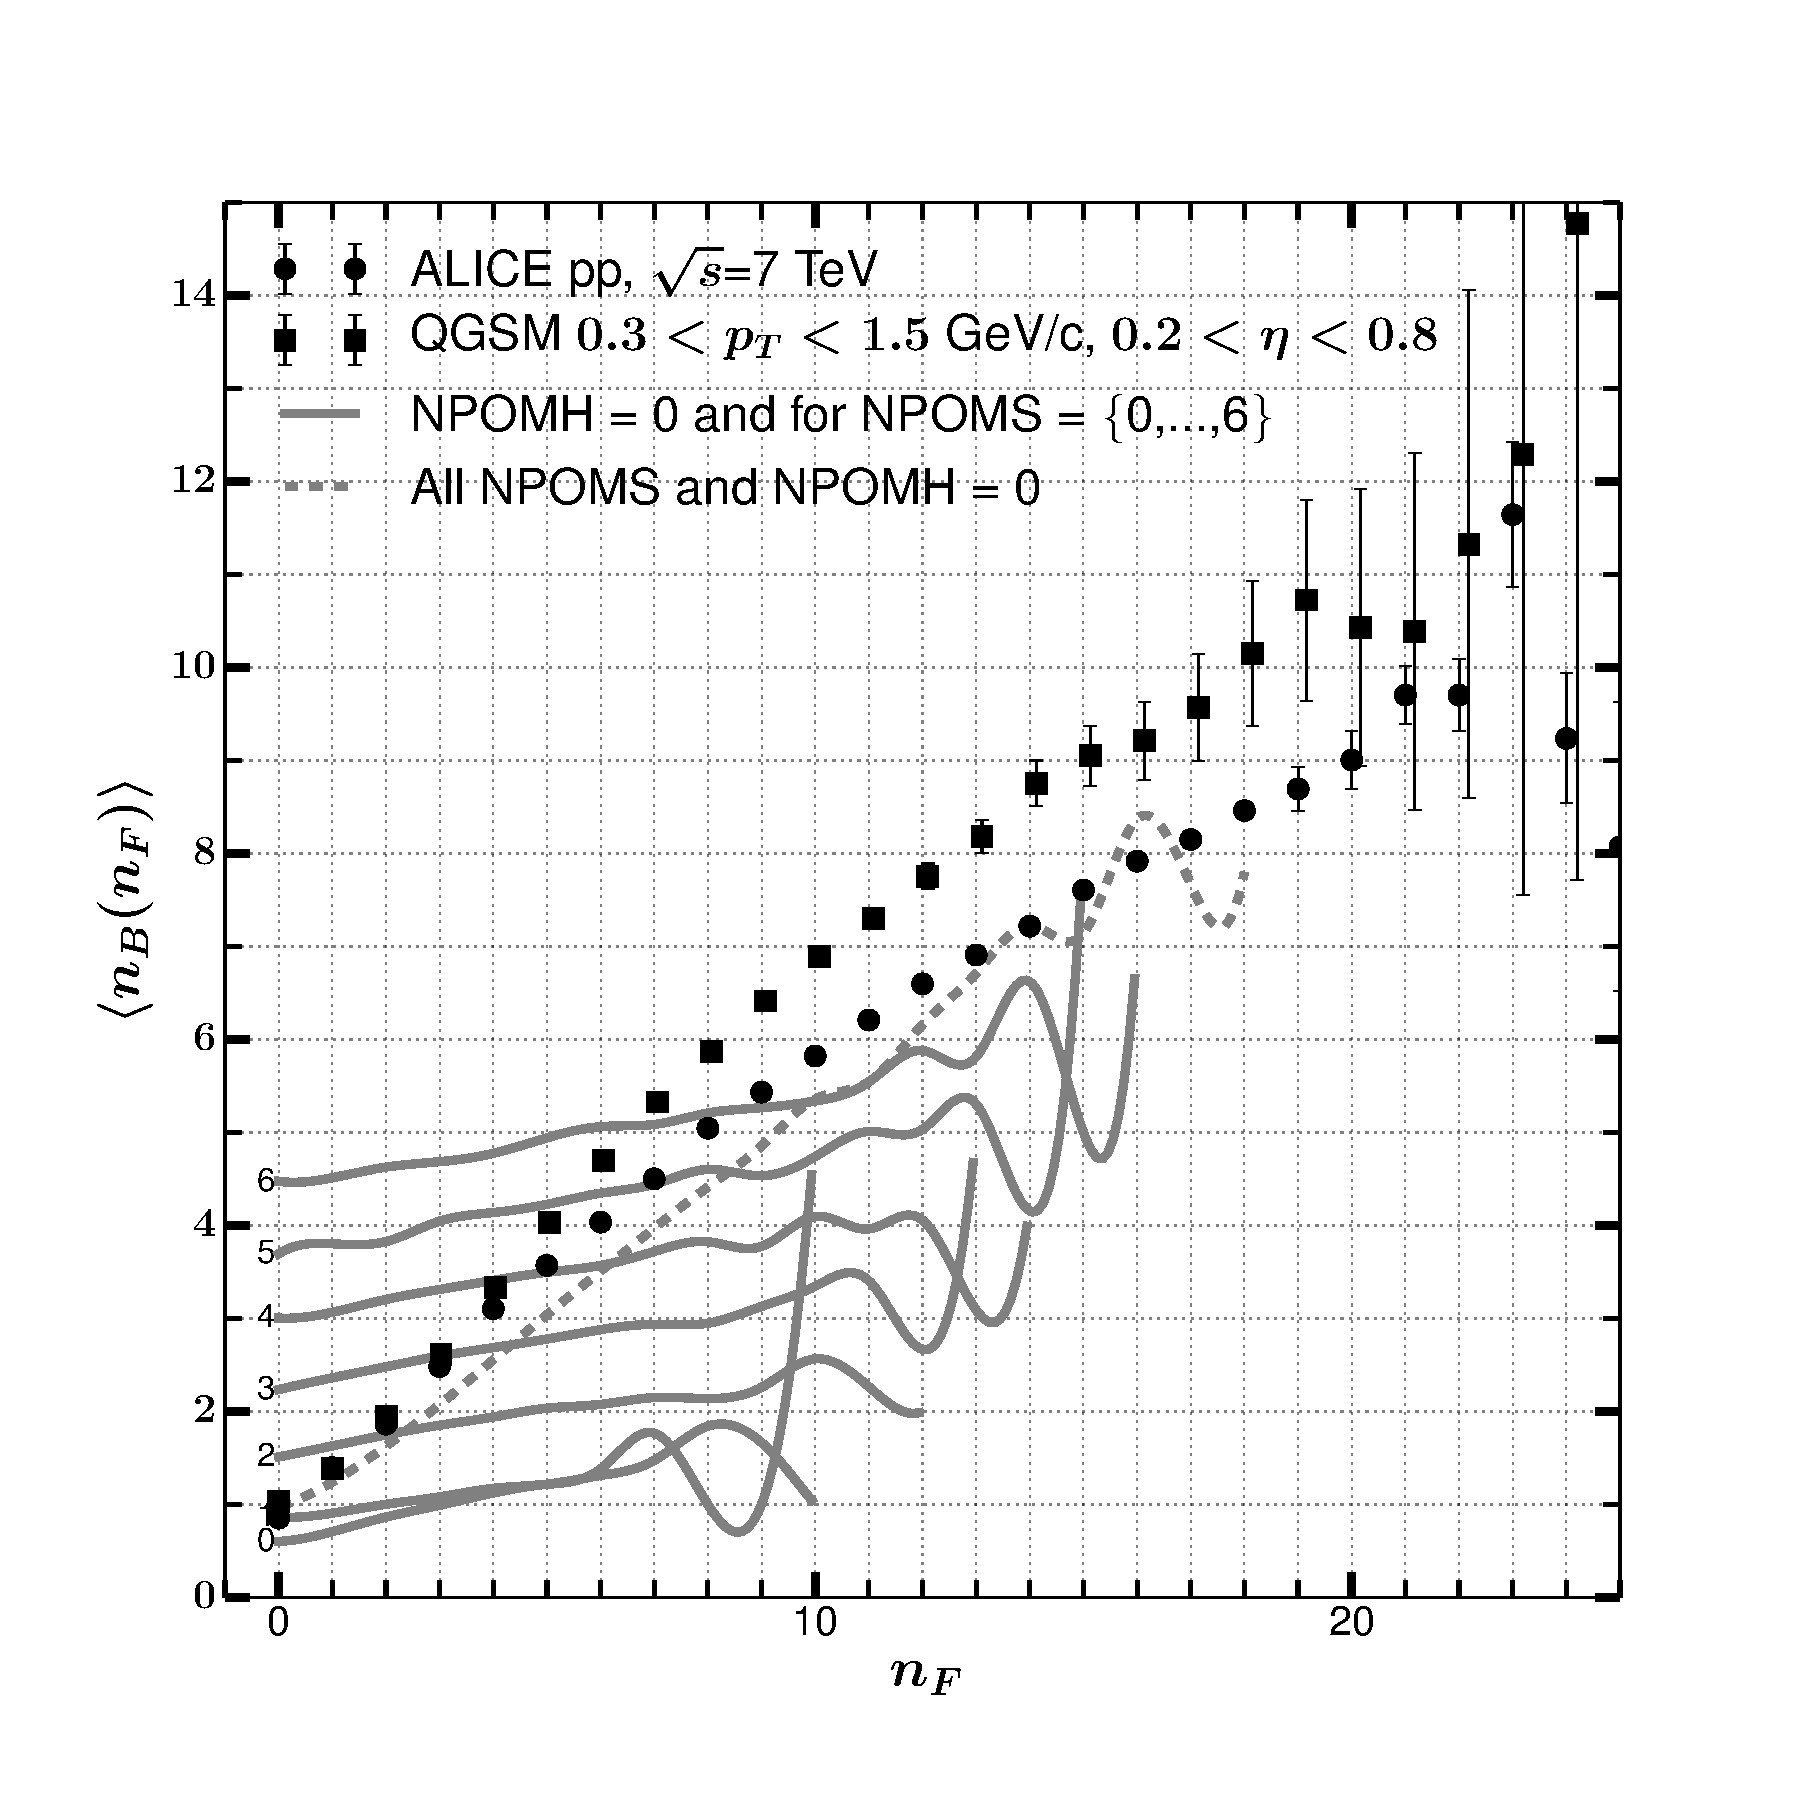
\includegraphics[scale=0.5]{../analyzed/nbnf_allnpoms_0npomh.pdf}
    \caption[All NPOMS and NPOMH=0]{}
\end{figure}

\begin{table}[h!]
\centering
    \begin{tabular}{|l|l|l|c|l|l|l|l|}
        \hline
Label     & a      & b     &     & $\eta_{gap}$ & $\delta\eta$ &Exp. $b_{corr}$ &Sim. $b_{corr}$\\\hline
Exp. fit  & 0.918  & 0.555 &     & 0.0 		    & 0.2 		   &0.366  		    &0.360\\\hline
All NPOMS &	0.961  & 0.550 &	 & 0.2 			& 0.2 		   &0.358  		    &0.358\\\hline 
$N = 8$	  &	0.97   & 0.533 &	 & 0.4 			& 0.2 		   &0.345  		    &0.353\\\hline
$N = 7$	  &	0.9761 & 0.517 &	 & 0.6 			& 0.2 		   &0.334  		    &0.348\\\hline
$N = 6$	  &	0.9836 & 0.493 &	 & 0.8 			& 0.2 		   &0.327  		    &0.343\\\hline
$N = 5$	  &	0.9911 & 0.454 &	 & 1.0 			& 0.2 		   &0.316  		    &0.337\\\hline
$N = 4$	  &	0.9928 & 0.398 &	 & 1.2 			& 0.2 		   &0.311  		    &0.334\\\hline
$N = 3$	  &	0.9775 & 0.323 &	 & 0.0 			& 0.4 		   &0.521  		    &0.524\\\hline
$N = 2$	  &	0.9249 & 0.227 &	 & 0.4 			& 0.4 		   &0.487  		    &0.511\\\hline
$N = 1$	  &	0.7992 & 0.116 &	 & 0.8 			& 0.4 		   &0.463  		    &0.496\\\hline
		  &	  	   &       &	 & 0.0			& 0.6		   &0.598		    &0.615\\\hline
	      &        &       &     & 0.4 			& 0.6 		   &0.564  		    &0.597\\\hline
		  &	  	   &       &	 & 0.0 			& 0.8 		   &0.643  		    &0.669\\\hline
    \end{tabular}
\caption[b correlation table]{}
\end{table}

\newpage
\subsubsection*{\centering N NPOMS and all NPOMH}

\begin{figure}[h!]
\centering
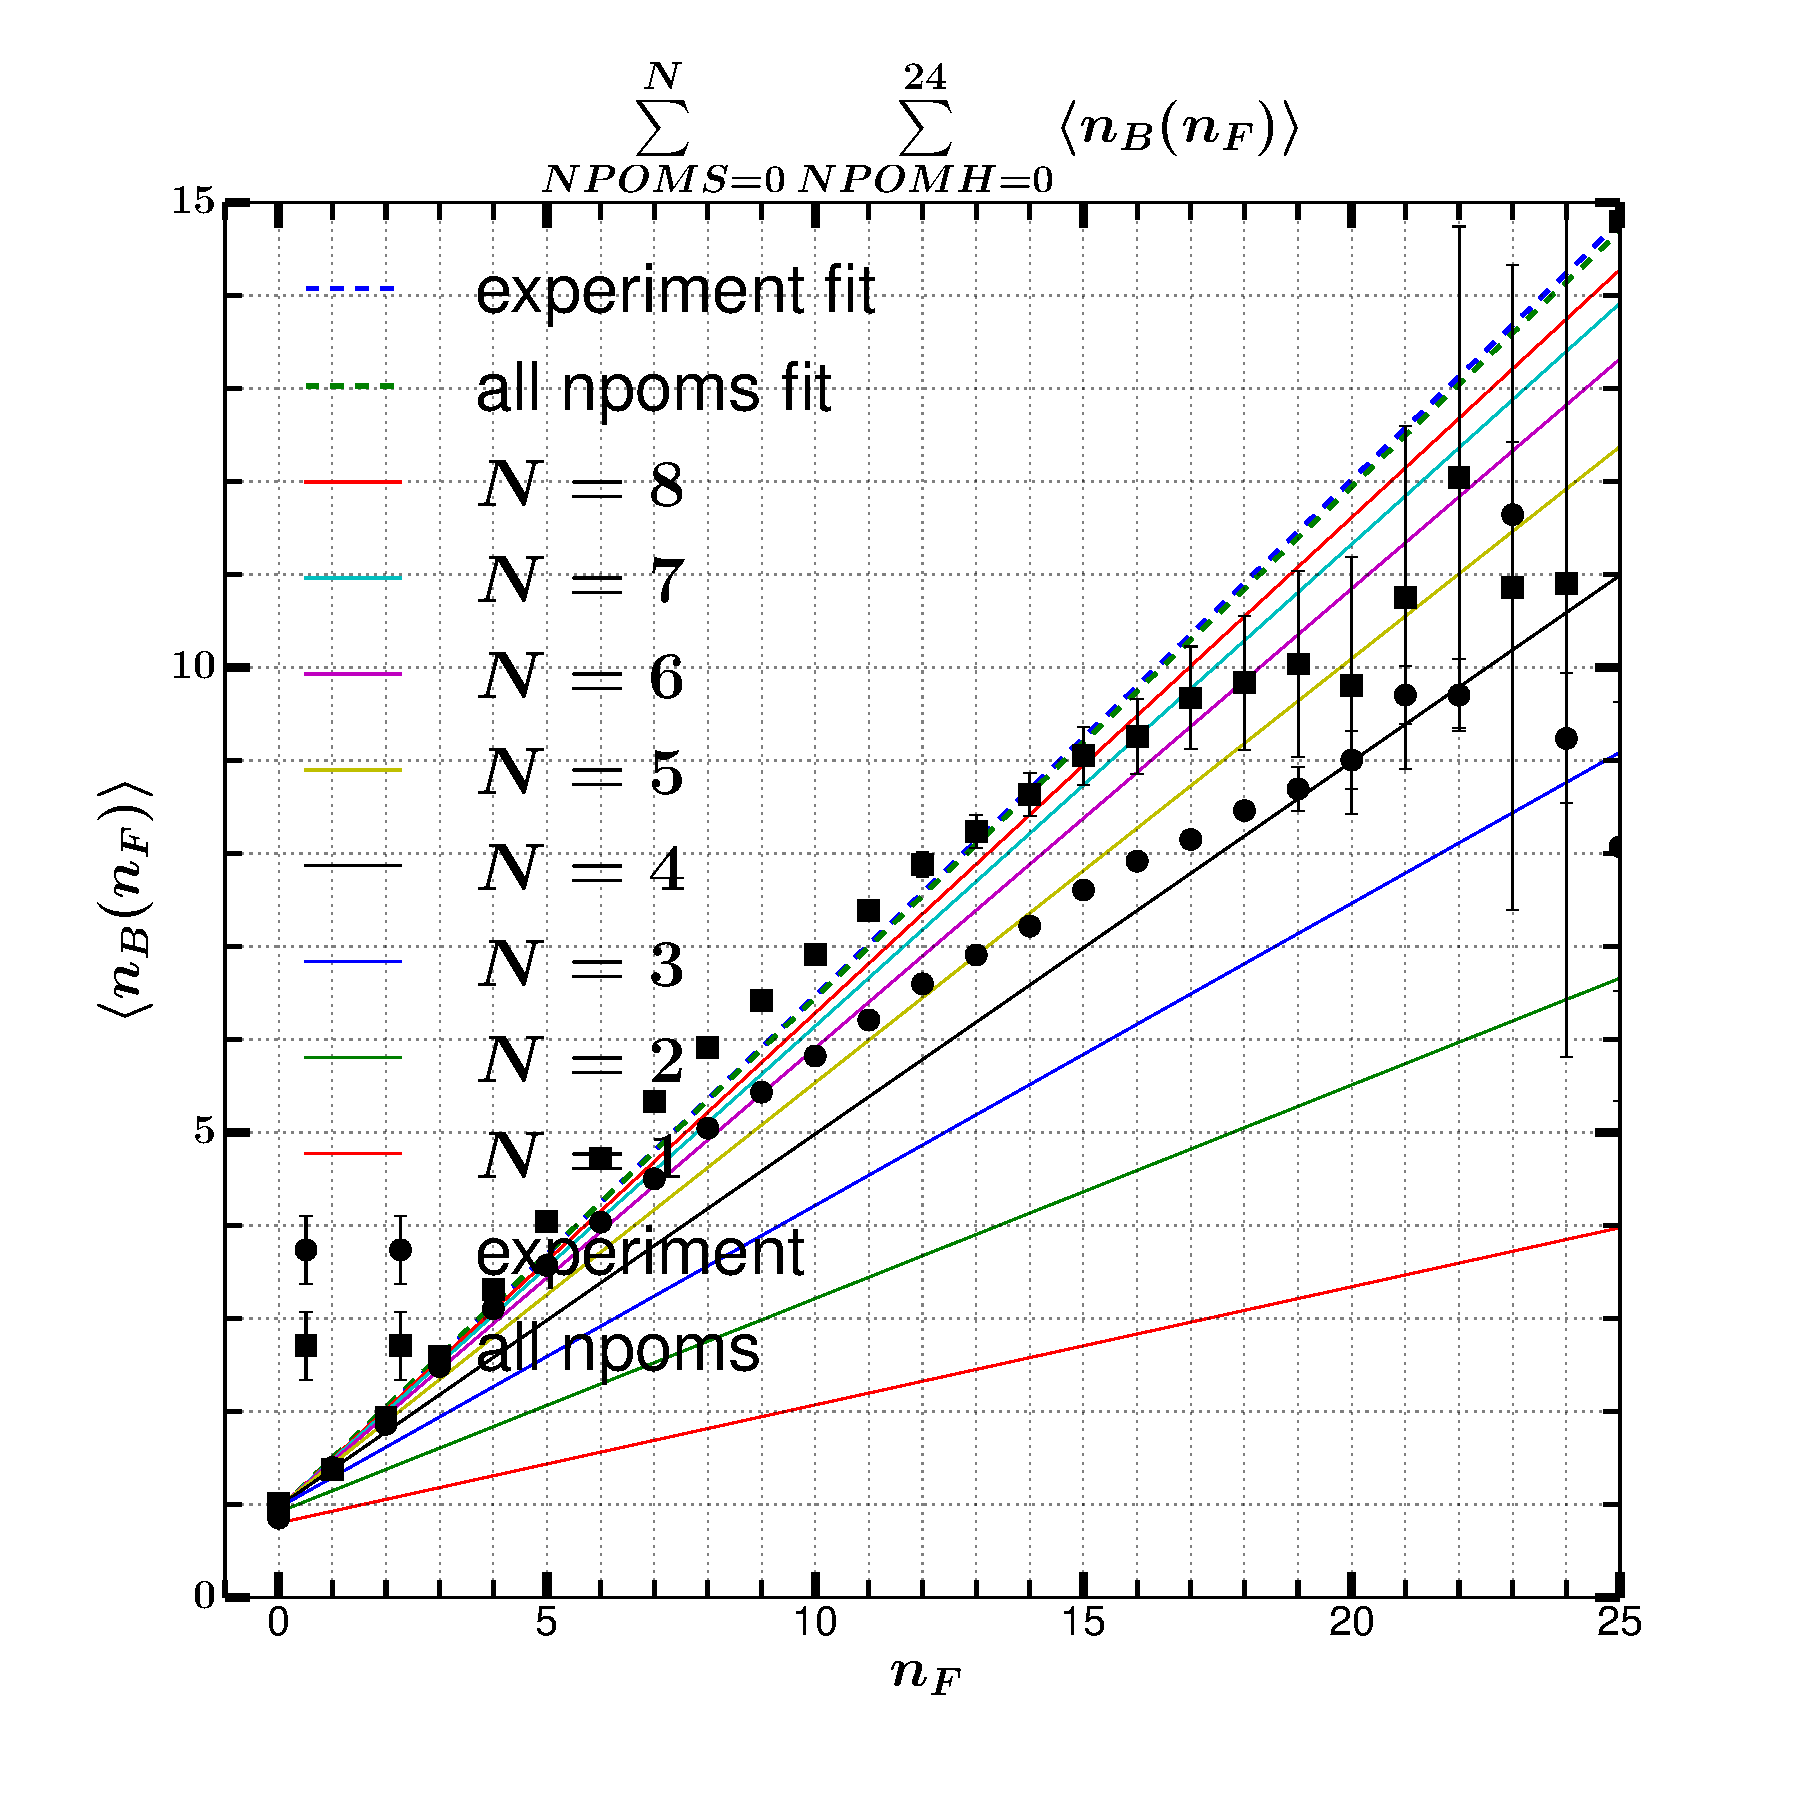
\includegraphics[scale=0.5]{../analyzed/nbnf_Nnpoms_allnpomh.pdf}
    \label{fig1}
    \caption[N NPOMS and all NPOMH]{}
\end{figure}

\newpage
\subsubsection*{\centering Fixed NPOMS and varying NPOMH}

\begin{figure}[h!]
    \centering
    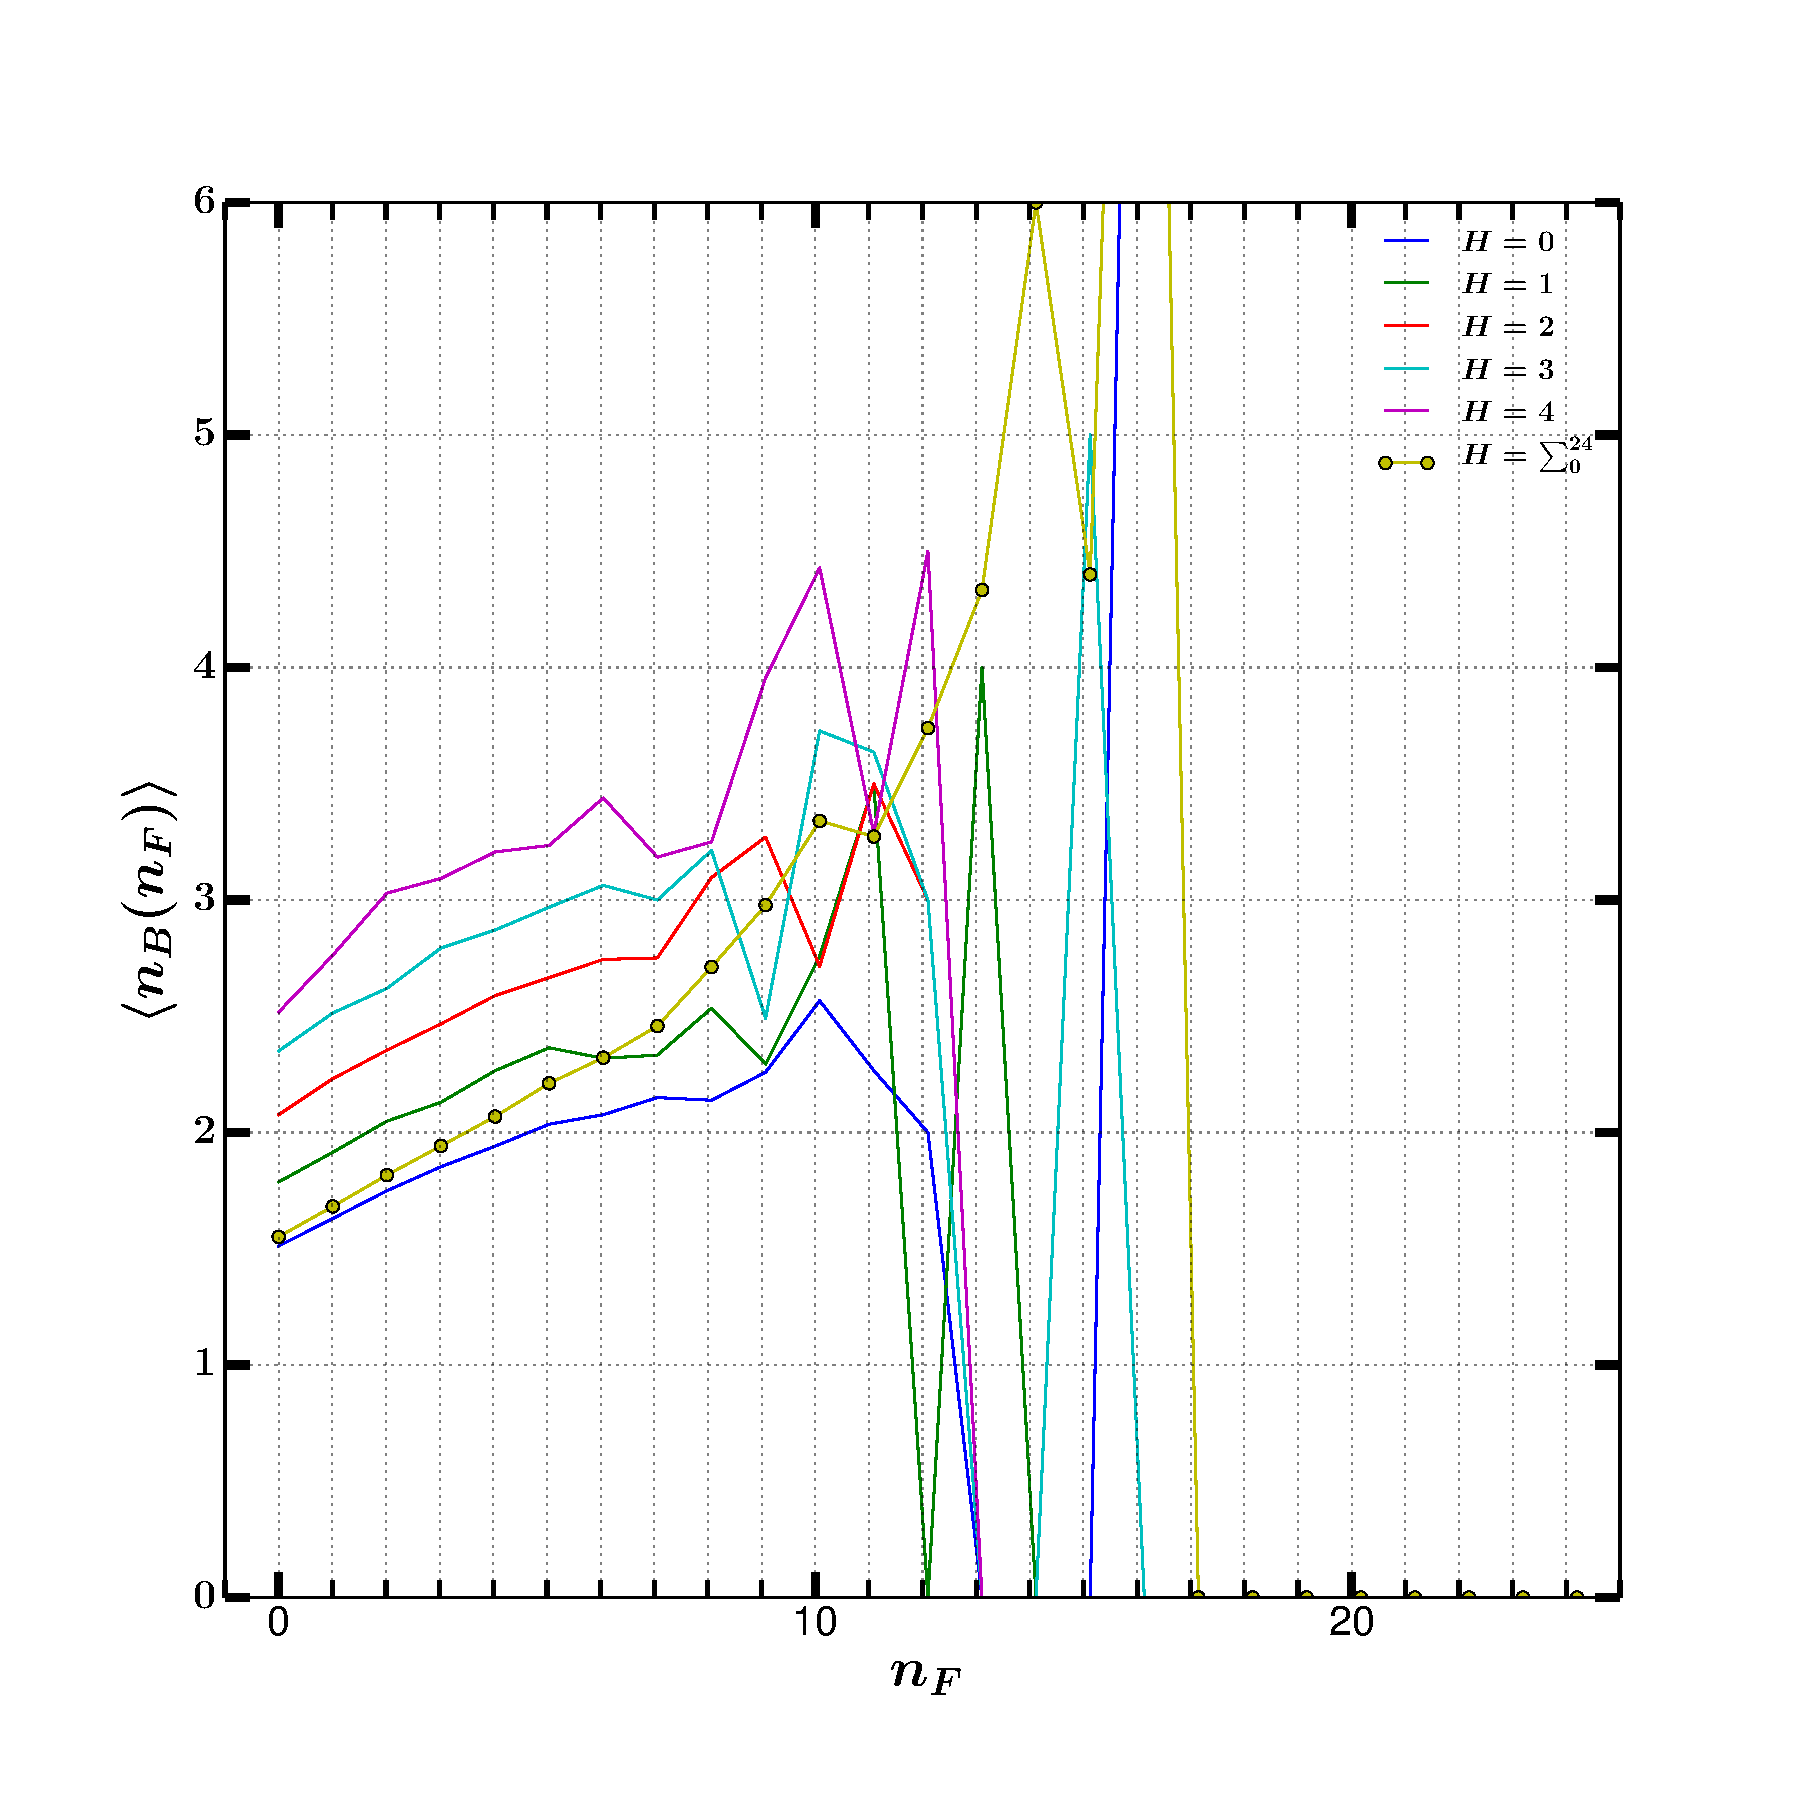
\includegraphics[scale=0.5]{../analyzed/nbnf_fixed_s_var_h.pdf}
    \caption[Fixed NPOMS and varying NPOMH]{}
\end{figure}

\newpage

\section*{\centering Non-Single diffraction, all diagrams except 1,4,6 and 10}

\subsubsection*{\centering N NPOMS and all NPOMH}
\begin{figure}[h!]
\centering
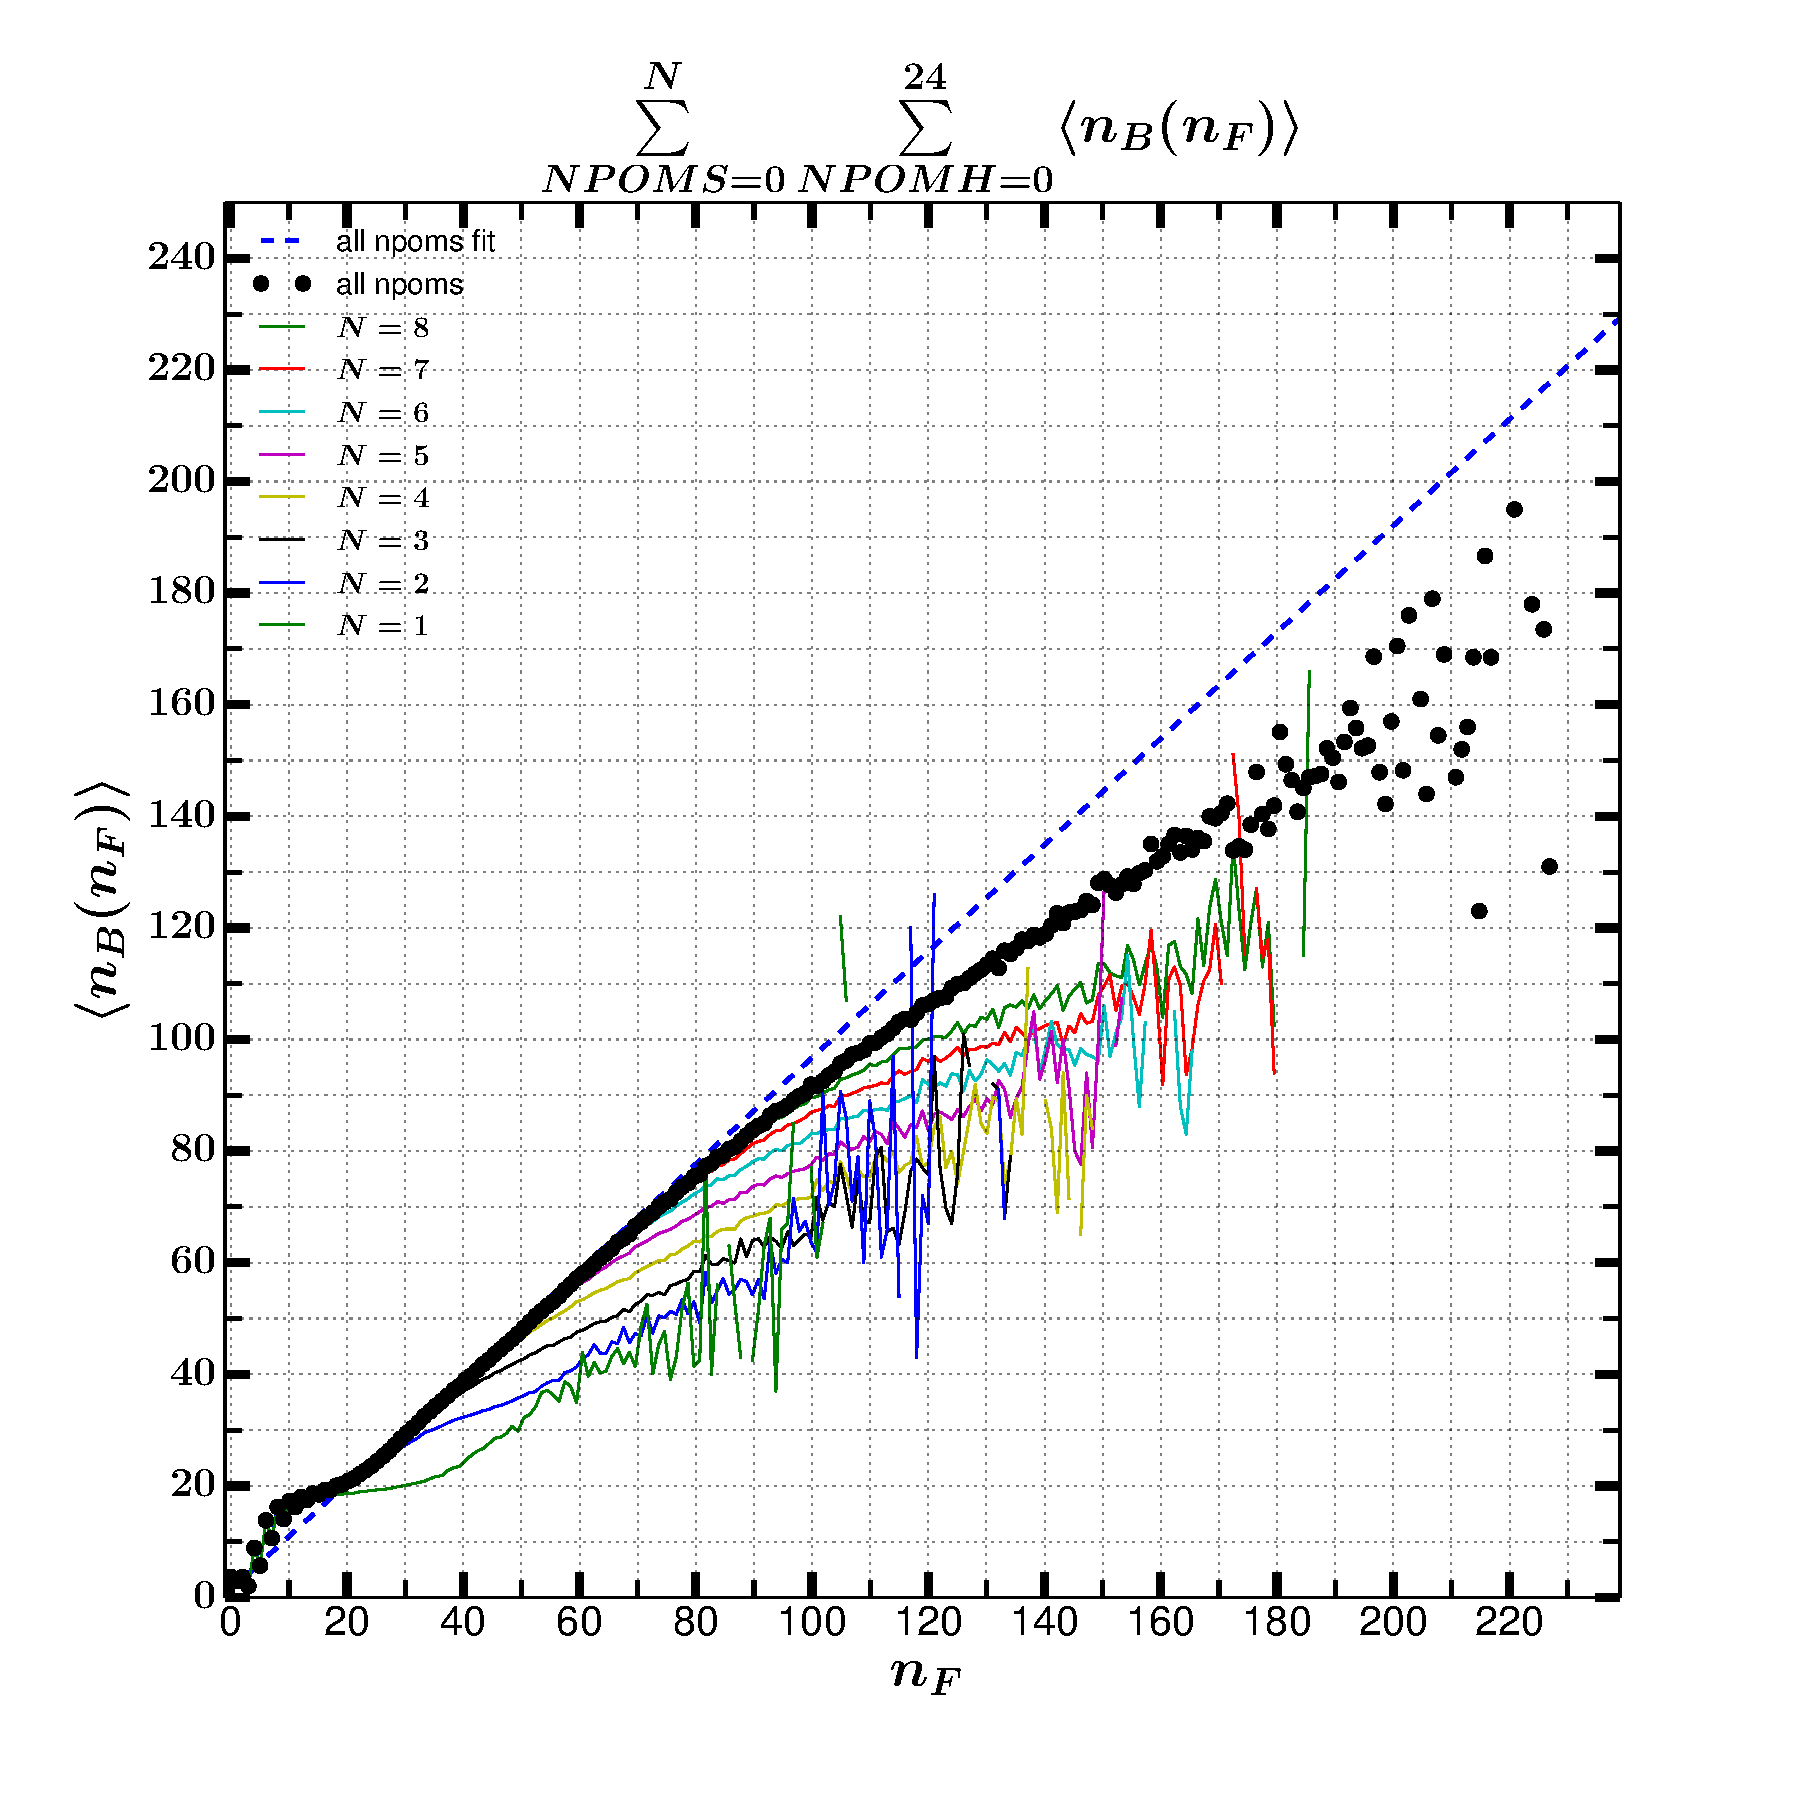
\includegraphics[scale=0.5]{../analyzed/nsd_nbnf_Nnpoms_allnpomh.pdf}
    \caption[NSD All NPOMS and NPOMH=0]{}
\end{figure}

\newpage
\subsubsection*{\centering All NPOMS and NPOMH=0}

\begin{figure}[h!]
    \centering
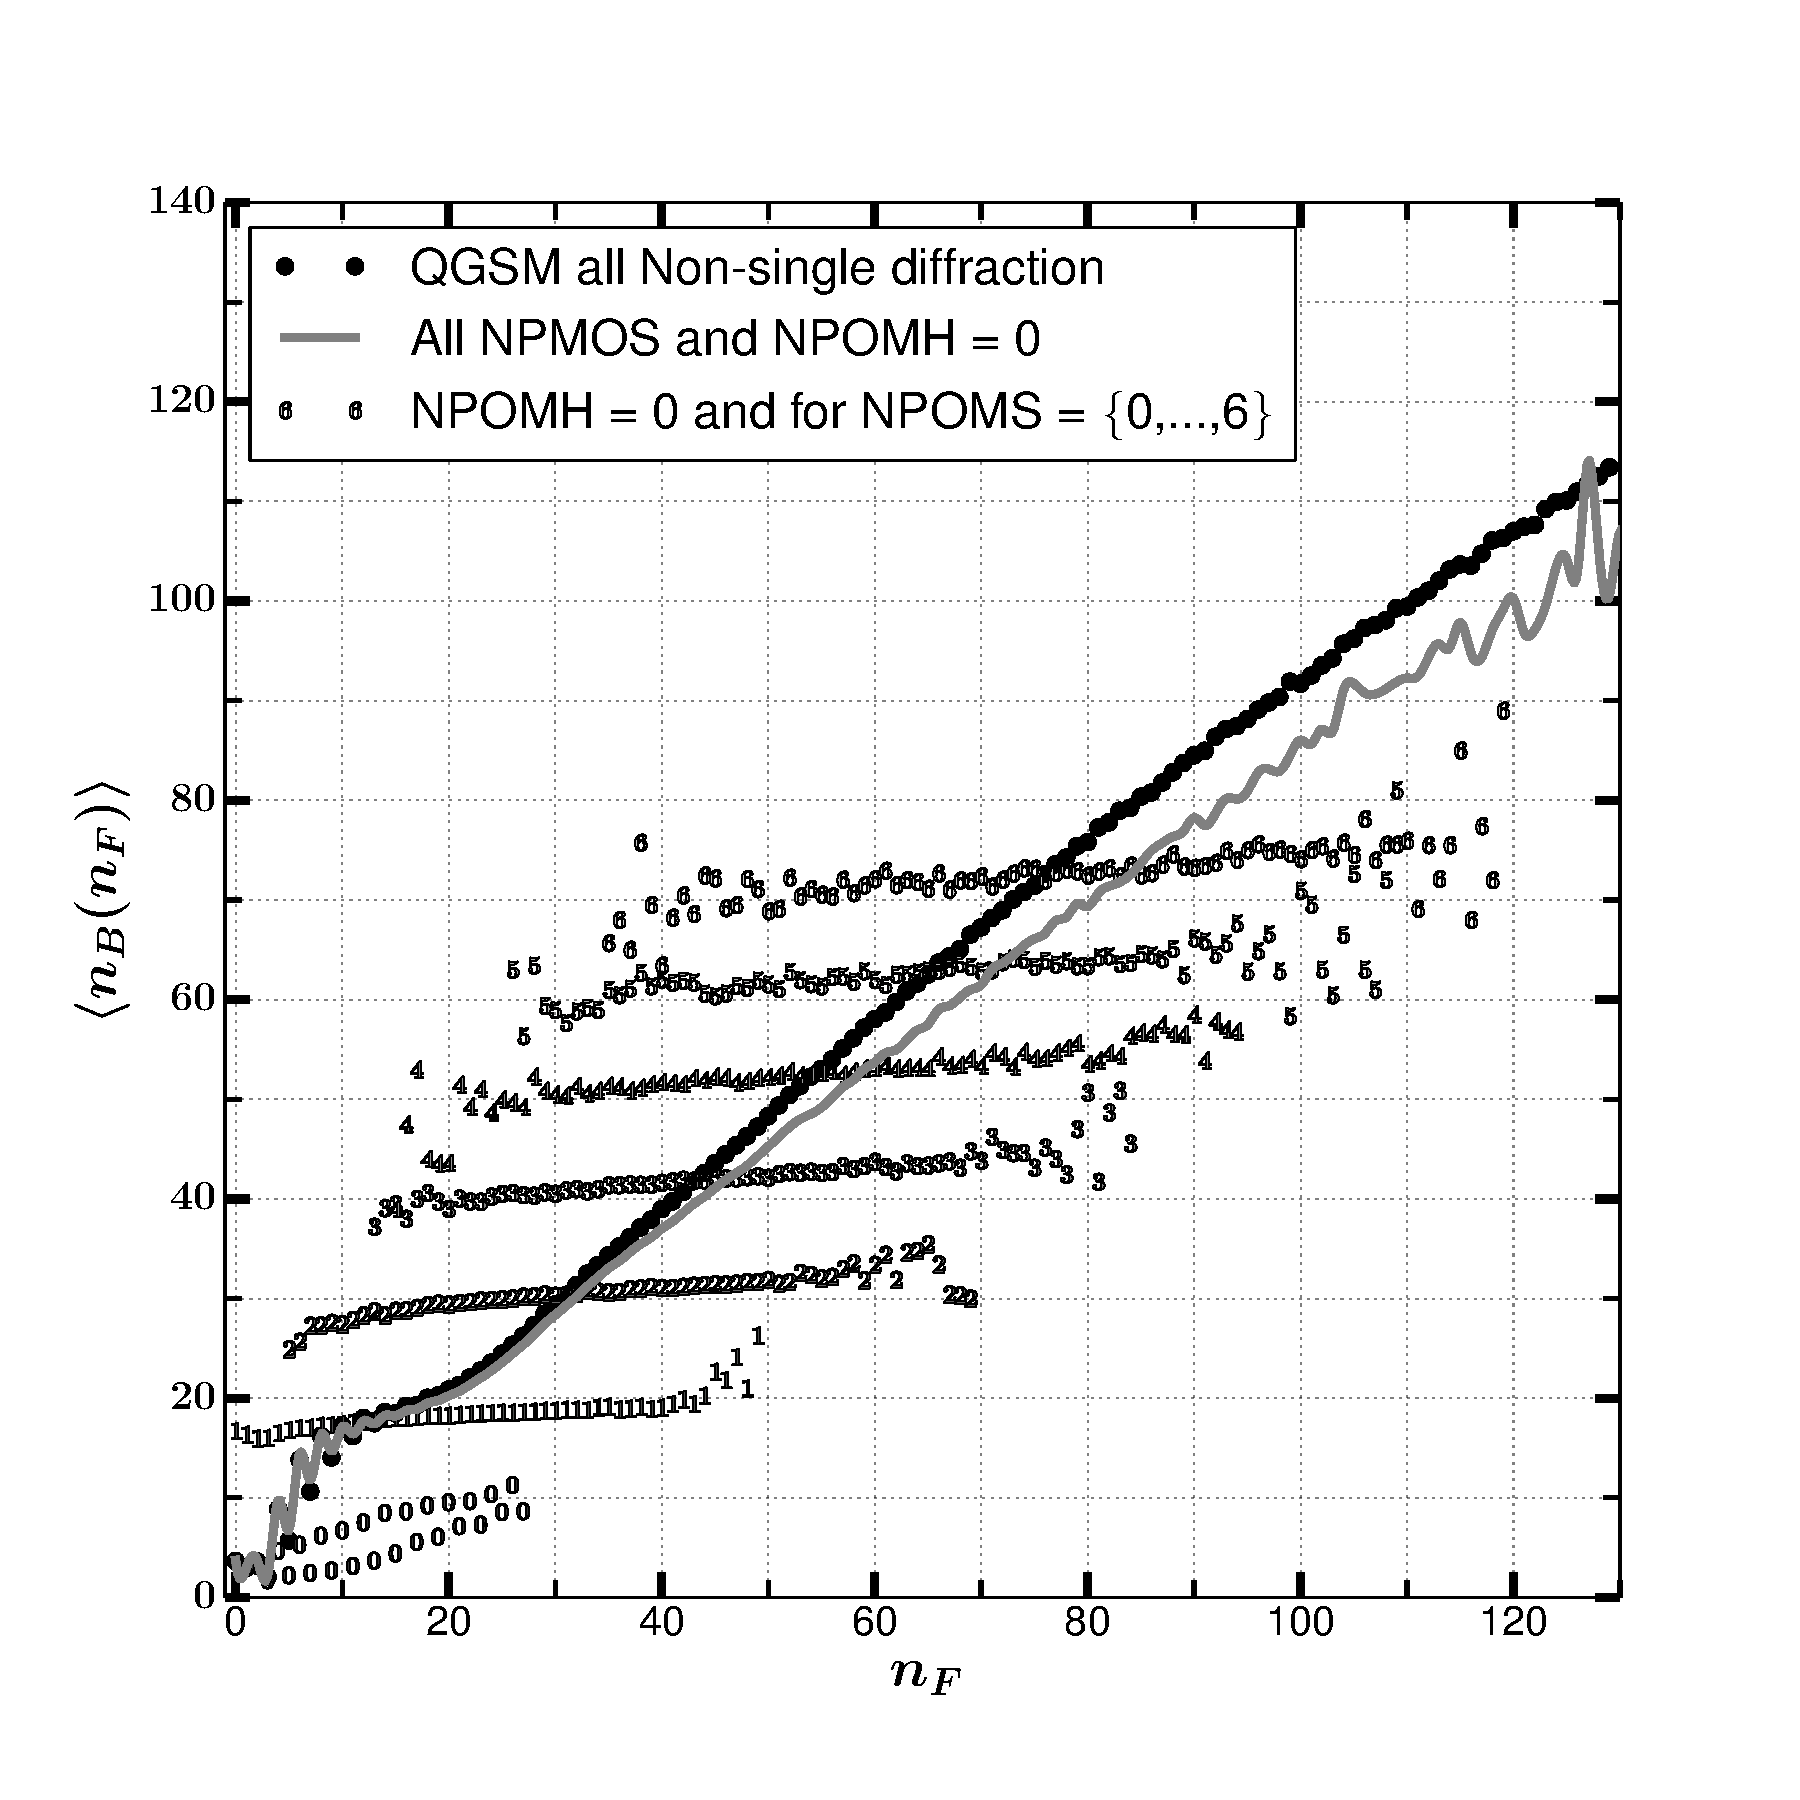
\includegraphics[scale=0.5]{../analyzed/nsd_nbnf_allnpoms_0npomh.pdf}
    \caption[NSD N NPOMS and all NPOMH]{}
\end{figure}

\newpage
\subsubsection*{\centering Fixed NPOMS and varying NPOMH}

\begin{figure}[h!]
    \centering
    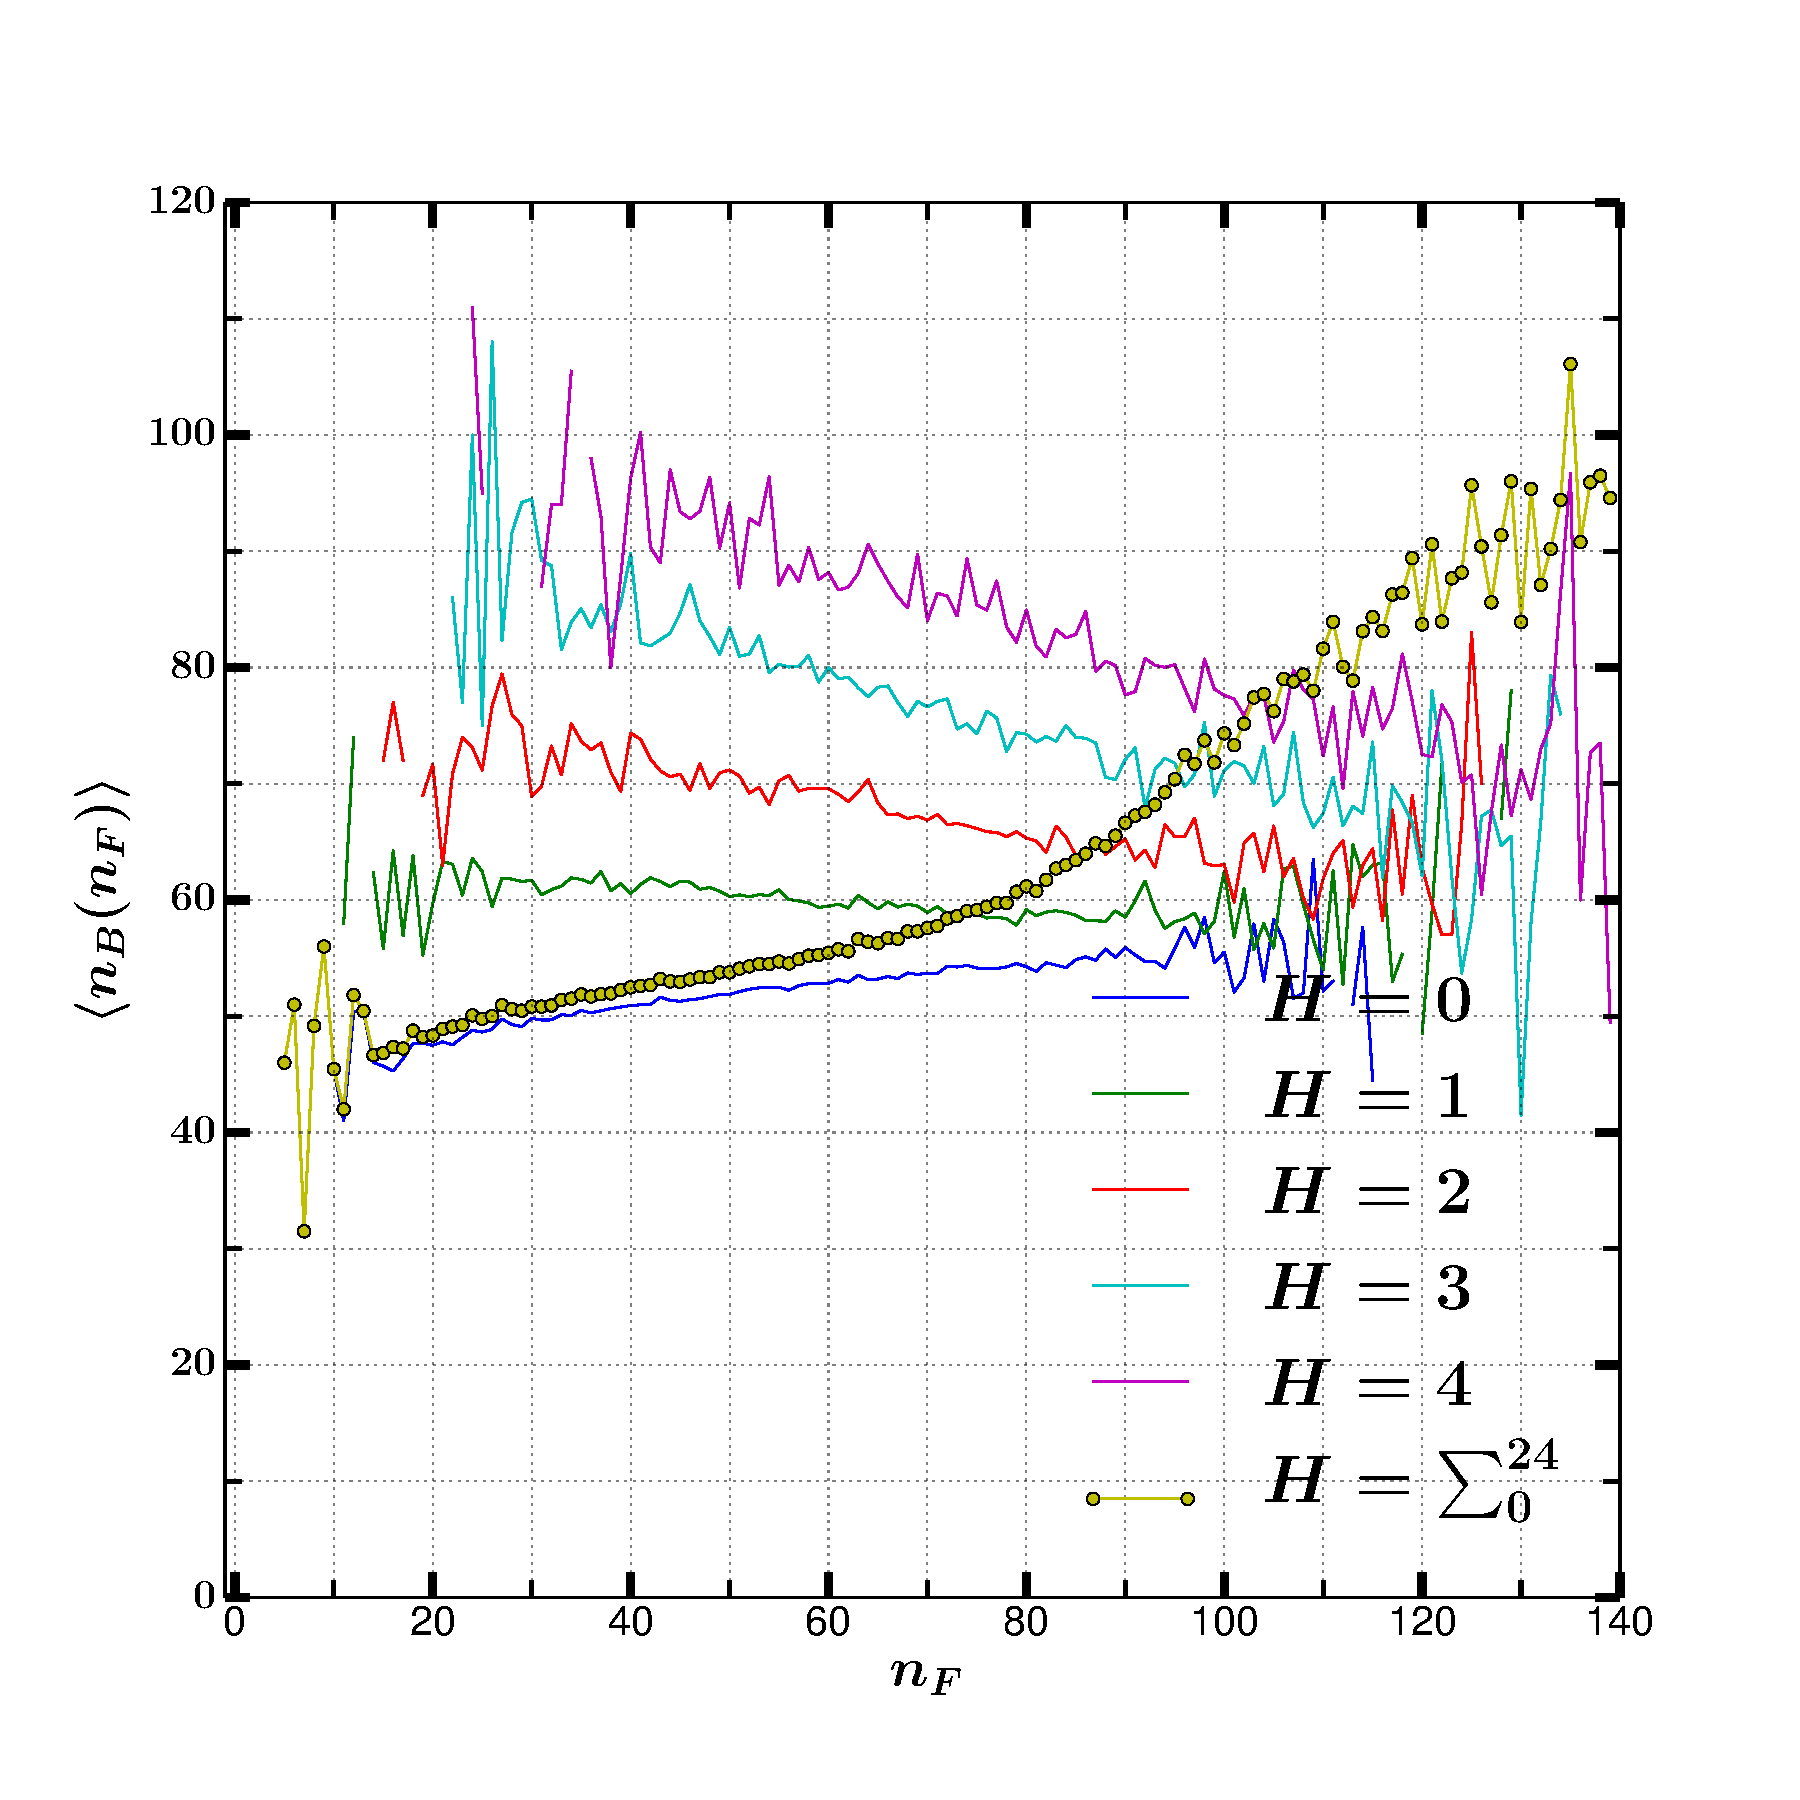
\includegraphics[scale=0.5]{../analyzed/nsd_nbnf_fixed_s_var_h.pdf}
    \caption[NSD Fixed NPOMS and varying NPOMH]{}
\end{figure}


\end{document}
